\documentclass[aspectratio=169]{beamer}

\usetheme{Madrid}
\usecolortheme{dolphin}

\usepackage{amsmath}
\usepackage{bm}

\usepackage{tikz}
\usepackage{pgfplots}
\pgfplotsset{compat=1.17} % Or your current version
\usetikzlibrary{shapes, arrows, positioning, fit}

\begin{document}


\title{Probabilistic Inference}
\subtitle{Approximate Inference: MC, MCMC, and VI}
\author{}
\date{}

\begin{frame}
  \titlepage
\end{frame}





\begin{frame}{Probabilistic inferences: Problem}
  \textbf{The world is noisy and partially observed.}
  \begin{itemize}
    \item We rarely observe the underlying mechanisms (diseases, customer preferences, physical laws) directly.
    \item We only observe their noisy effects (symptoms, clickstreams, measurements).
  \end{itemize}

  \vspace{0.6em}
  Probabilistic inference provides the tools to quantify and reason about this uncertainty. It moves us beyond point estimates to understanding distributions and making predictions with confidence intervals. This is essential for real-world applications where risk assessment and understanding the range of possible outcomes are critical (e.g., medical diagnosis, financial forecasting, autonomous driving).
\end{frame}

\begin{frame}{Uncertainty in healthcare: why it matters}

      \centering
      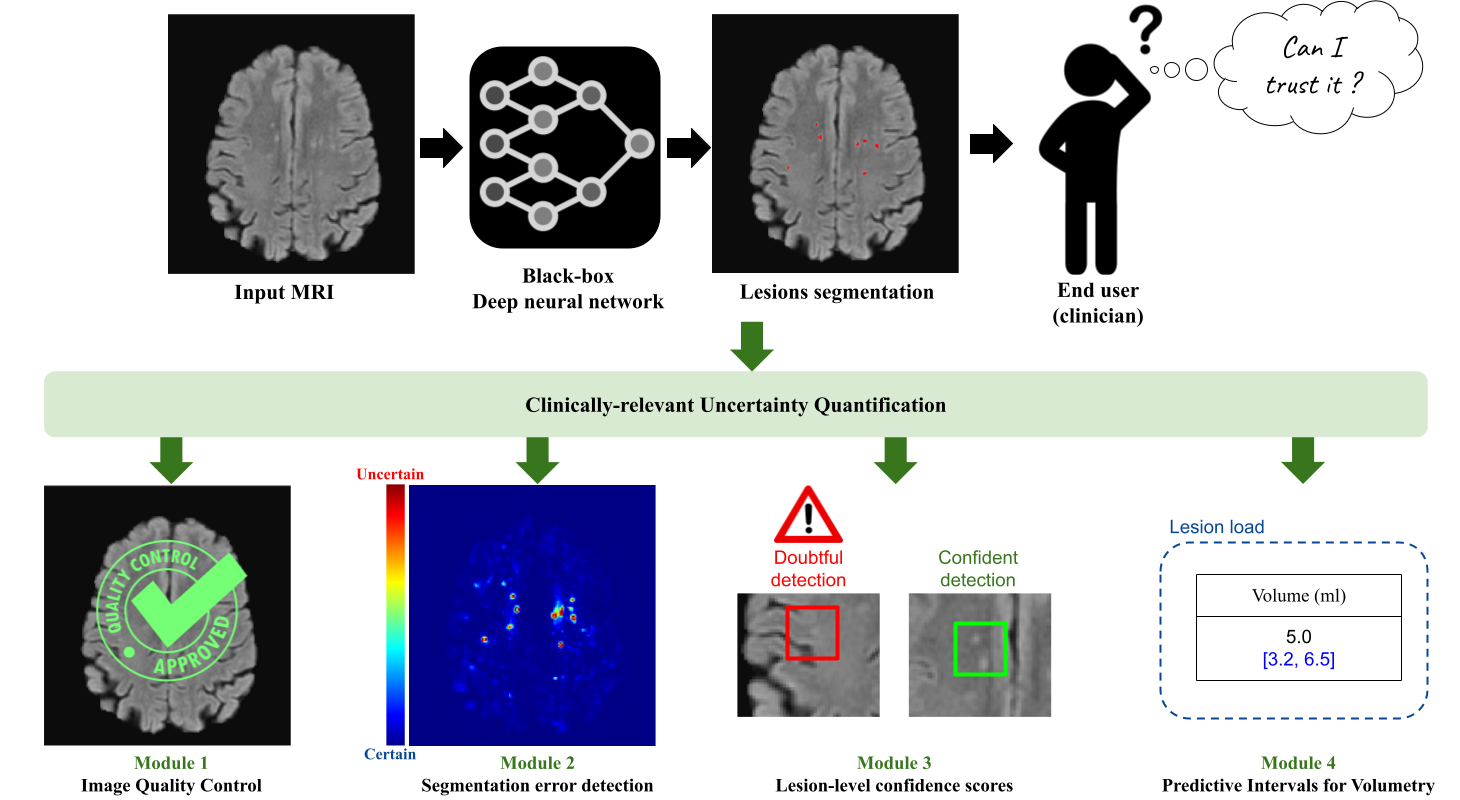
\includegraphics[width=0.8\linewidth]{Figures/uncer.png}

      \footnotesize{https://neurosciences.univ-grenoble-alpes.fr/en/news/uncertainty-quantification-deep-learning-based-medical-image-segmentation
}


\end{frame}


\begin{frame}{The Bayesian Framework}
  \textbf{Bayes' Rule} is the mechanical engine for this inversion.
  It tells us how to update our belief about hypothesis $H$ (or parameters $\theta$) given evidence $E$ (or data $\bm{x}$).

  \[
    \underbrace{p(\theta \mid \bm{x})}_{\text{Posterior}}
    \;=\;
    \frac{\overbrace{p(\bm{x} \mid \theta)}^{\text{Likelihood}} \, \overbrace{p(\theta)}^{\text{Prior}}}
         {\underbrace{p(\bm{x})}_{\text{Evidence}}}
  \]

  \begin{itemize}
    \item \textbf{Prior $p(\theta)$:} Belief before seeing data (domain knowledge).
    \item \textbf{Likelihood $p(\bm{x} \mid \theta)$:} How well parameters explain the data.
    \item \textbf{Posterior $p(\theta \mid \bm{x})$:} Updated belief (the goal of inference).
    \item \textbf{Evidence $p(\bm{x})$:} Normalizing constant (ensures probabilities sum to 1).
  \end{itemize}
\end{frame}


\begin{frame}{Probabilistic inference: what and why}
  \textbf{Goal:} compute the \textbf{posterior} over latent variables/parameters given data
  \[
    p(\theta, \bm{z}\mid \bm{x})
    \;=\;
    \frac{p(\bm{x}\mid \bm{z},\theta)\,p(\bm{z}\mid \theta)\,p(\theta)}
         {p(\bm{x})},
    \qquad
    p(\bm{x})=\int\!\!\int p(\bm{x},\bm{z},\theta)\,d\bm{z}\,d\theta.
  \]

  \vspace{0.4em}
  \textbf{In healthcare DS:} uncertainty-aware prediction and decision support
  \begin{itemize}
    \item Missingness, measurement noise, small cohorts $\Rightarrow$ quantify uncertainty.
    \item Interpretability: latent phenotypes/subtypes, disease progression states.
    \item Downstream: credible intervals, posterior predictive checks, risk stratification.
  \end{itemize}
\end{frame}

\begin{frame}{Probabilistic inference: what and why}
  The numerator (Likelihood $\times$ Prior) is usually easy to compute.
  The denominator (Evidence) is the bottleneck.

  \[
    p(\bm{x})=\int\!\!\int p(\bm{x},\bm{z},\theta)\,d\bm{z}\,d\theta.
  \]

  \begin{itemize}
    \item This integral sums over \emph{all possible configurations} of parameters/latents.
    \item In high dimensions (e.g., neural networks, complex hierarchical models), this integral is \textbf{analytically intractable}.
  \end{itemize}

  \vspace{0.4em}
  \textbf{The Challenge:} We need $p(\theta \mid \bm{x})$ to make decisions, but we cannot compute the denominator directly. This necessitates \textbf{Approximate Inference}.
\end{frame}


%%%%%%%%%%%%%%%%%%%%%%%%%%%%%%%%%%%%%%%%%%%%%%%%%%%%%%%%%%%%%%%%%%%%%%%

\begin{frame}{Overview: types of inference (in practice)}
  \begin{itemize}
    \item \textbf{Exact inference}:
      compute posterior quantities exactly (closed-form or exact algorithms).
      \\[-0.2em]\begin{itemize}
        \item Works for conjugate models or low-treewidth graphs; becomes intractable at scale.
      \end{itemize}
    \item \textbf{Approximate inference}:
      trade bias/variance and compute for tractability.
      \\[-0.2em]\begin{itemize}
        \item \textbf{MC}: estimate expectations with samples (when sampling is feasible).
        \item \textbf{MCMC}: build a Markov chain to sample from the posterior (often accurate, slower).
        \item \textbf{VI}: optimize a simpler $q_\phi$ to approximate the posterior (fast, can be biased).
      \end{itemize}
  \end{itemize}
\end{frame}

\begin{frame}{Exact inference}
  \textbf{Exact inference} computes posterior quantities \emph{without approximation} (when tractable).
  \begin{itemize}
  \item \textbf{Brute-force:}
    \item \textbf{Conjugate models:} closed-form posteriors (e.g., Beta--Binomial, Normal--Normal).
    \item \textbf{Variable elimination:} exact marginals in graphical models
          (efficient mainly on trees / low treewidth).
    \item \textbf{Limitations:} high-dimensional integrals/sums, complex likelihoods,
          non-conjugacy, large datasets.
  \end{itemize}

  \vspace{0.4em}
  \textbf{When exact works:} small or structured models; good for sanity checks and baselines.
\end{frame}




\begin{frame}{Approximate inference: the big picture}
  When exact inference is intractable, approximate inference targets one or more of:
  \begin{itemize}
    \item \textbf{Posterior summaries:} $\mathbb{E}[f(\theta,\bm{z})\mid \bm{x}]$ (What is the average value?), marginals, quantiles.
    \item \textbf{Posterior predictive:} $p(\tilde{\bm{x}}\mid \bm{x})=\int p(\tilde{\bm{x}}\mid \theta)\,p(\theta\mid \bm{x})\,d\theta$ (To predict future data).
  \end{itemize}

  \vspace{0.6em}
  \textbf{Three common families (this course):}
  \begin{enumerate}
    \item \textbf{MC:} Monte Carlo integration (sampling from a known distribution).
    \item \textbf{MCMC:} Markov chain Monte Carlo (sampling from an unknown posterior).
    \item \textbf{VI:} Variational inference (optimization-based approximation).
  \end{enumerate}
\end{frame}

%%%%%%%%%%%%%%%%%%%%%%%%%%%%%%%%%%%%%%%%%%%%%%%%%%%%%%%%%%%%%%%%%%%%%%%%%%
%%%%%%%%%%%%%%%%%%%%%%%%%%%%%%%%%%%%%%%%%%%%%%%%%%%%%%%%%%%%%%%%%%%%%%%%%%
%%%%%%%%%%%%%%%%%%%%%%%%%%%%%%%%%%%%%%%%%%%%%%%%%%%%%%%%%%%%%%%%%%%%%%%%%%


\begin{frame}[plain]
    \centering
    \vfill
    {\usebeamerfont{section title}Monte Carlo (MC) \par}
    \vfill
  \end{frame}


\begin{frame}{Monte Carlo (MC): layman explanation}
  \textbf{Big idea:} when an average is hard to compute exactly, \emph{estimate it by repeated random trials}.

  \vspace{0.4em}
  \begin{itemize}
    \item Think: you want the ``typical'' outcome, but the process is noisy/uncertain.
    \item You simulate (or draw) many plausible outcomes from the model, like running the same experiment many times.
    \item You then \textbf{average} what you care about across those simulated outcomes.
  \end{itemize}


  \vspace{0.4em}
  \textbf{Rule of thumb:} more samples $\Rightarrow$ more stable estimates (but more compute).
\end{frame}

\begin{frame}{Monte Carlo (MC)}
  \textbf{Use case:} estimate expectations under a distribution you can sample from.
  \[
    \mathbb{E}_{p}[f(\theta)]
    \approx
    \frac{1}{S}\sum_{s=1}^S f(\theta^{(s)}), \quad \theta^{(s)}\sim p(\theta).
  \]
  \begin{itemize}
    \item Error decreases as $O(S^{-1/2})$ (dimension-free, but can be slow).
    \item \textbf{Importance sampling:} sample from proposal $q$ and reweight to target $p$.

  \end{itemize}
\end{frame}



\begin{frame}{MC example: approximating an expectation}
  \textbf{Goal:} approximate $\mathbb{E}[f(z)]$ with Monte Carlo samples, where
  $f(z)=z^2$ and $z\sim \mathrm{Uniform}(0,1)$.

  \vspace{0.4em}
  \textbf{True value (exact inference):}
  \[
    \mathbb{E}[z^2]
    =
    \int_{0}^{1} z^2\,dz
    =
    \left[\frac{z^3}{3}\right]_{0}^{1}
    =
    \frac{1}{3}.
  \]

  \vspace{0.4em}
  \textbf{MC estimator:}
  \[
    \widehat{\mathbb{E}}[z^2]
    =
    \frac{1}{S}\sum_{s=1}^{S}\left(z^{(s)}\right)^2,
    \qquad
    z^{(s)} \stackrel{i.i.d.}{\sim} \mathrm{Uniform}(0,1).
  \]

  \vspace{0.2em}
  \textbf{Key takeaway:} as $S$ increases, $\widehat{\mathbb{E}}[z^2]\to 1/3$ (error $\sim O(S^{-1/2})$).
\end{frame}


\begin{frame}{Importance sampling (IS)}
  \textbf{Goal:} estimate expectations under a target $p(\theta)$ when direct sampling is hard,
  using samples from an easier proposal $q(\theta)$.

  \vspace{0.4em}
  \textbf{Key identity:}
  \[
    \mathbb{E}_{p}[f(\theta)]
    =
    \int f(\theta)\,p(\theta)\,d\theta
    =
    \int f(\theta)\,\frac{p(\theta)}{q(\theta)}\,q(\theta)\,d\theta.
  \]

  \textbf{IS estimator:}
  \[
    \widehat{\mathbb{E}}_{p}[f(\theta)]
    =
    \frac{1}{S}\sum_{s=1}^{S} f(\theta^{(s)})\,w(\theta^{(s)}),
    \qquad
    \theta^{(s)}\sim q(\theta),
    \quad
    w(\theta)=\frac{p(\theta)}{q(\theta)}.
  \]

  \vspace{0.4em}
  \textbf{Self-normalized IS (common in practice):}
  \[
    \tilde{w}_s=\frac{w(\theta^{(s)})}{\sum_{j=1}^{S} w(\theta^{(j)})},
    \qquad
    \widehat{\mathbb{E}}_{p}[f(\theta)]
    \approx
    \sum_{s=1}^{S} \tilde{w}_s\, f(\theta^{(s)}).
  \]


\end{frame}


\begin{frame}{Importance sampling: illustration}
  \centering
  % Upload your image into the project (e.g., Figures/is_illustration.png)
  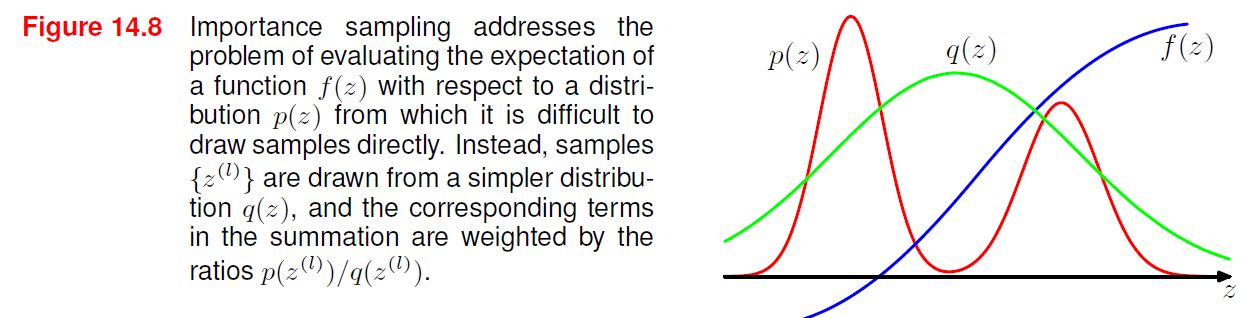
\includegraphics[width=0.9\linewidth]{Figures/import.png}
\end{frame}

%%%%%%%%%%%%%%%%%%%%%%%%%%%%%%%%%%%%%%%%%%%%%%%%%%%%%%%%%%%%%%%%%%%%%%%%%%
%%%%%%%%%%%%%%%%%%%%%%%%%%%%%%%%%%%%%%%%%%%%%%%%%%%%%%%%%%%%%%%%%%%%%%%%%%
%%%%%%%%%%%%%%%%%%%%%%%%%%%%%%%%%%%%%%%%%%%%%%%%%%%%%%%%%%%%%%%%%%%%%%%%%%

\begin{frame}[plain]
    \centering
    \vfill
    {\usebeamerfont{section title}Markov chain Monte Carlo (MCMC) \par}
    \vfill
  \end{frame}


\begin{frame}{Markov chain Monte Carlo (MCMC)}
  \textbf{Idea:} construct a Markov chain whose stationary distribution is the posterior.
  \begin{itemize}
    \item \textbf{Metropolis--Hastings:} propose $\theta'\sim r(\theta'\mid \theta)$, accept/reject.
    \item \textbf{Gibbs sampling:} iterate sampling from conditionals when available.
    \item \textbf{*Hamiltonian Monte Carlo (HMC/NUTS):} uses gradients to explore efficiently. (*common in ML/DL)
  \end{itemize}


\end{frame}



\begin{frame}{Metropolis--Hastings: layman explanation}
  \textbf{Big idea:} when you cannot draw perfect independent samples from the posterior,
  you take a \emph{guided random walk} that prefers more plausible values.

  \vspace{0.4em}
  \begin{itemize}
    \item Start with a reasonable guess for $\theta$.
    \item Propose a small random change (a ``nearby'' candidate).
    \item If the candidate explains the data better (higher posterior probability), accept it.
    \item If it explains the data worse, you \emph{might still accept it} sometimes---to avoid getting stuck.
    \item Repeating this many times produces a trail of values that spends more time in high-probability regions.
  \end{itemize}

  \vspace{0.4em}
  \textbf{Intuition:} like hiking in fog with a compass that biases you toward valleys (good fit),
  but occasionally lets you step uphill so you can find an even better valley later.
\end{frame}

\begin{frame}{MCMC: illustration}
  \centering
  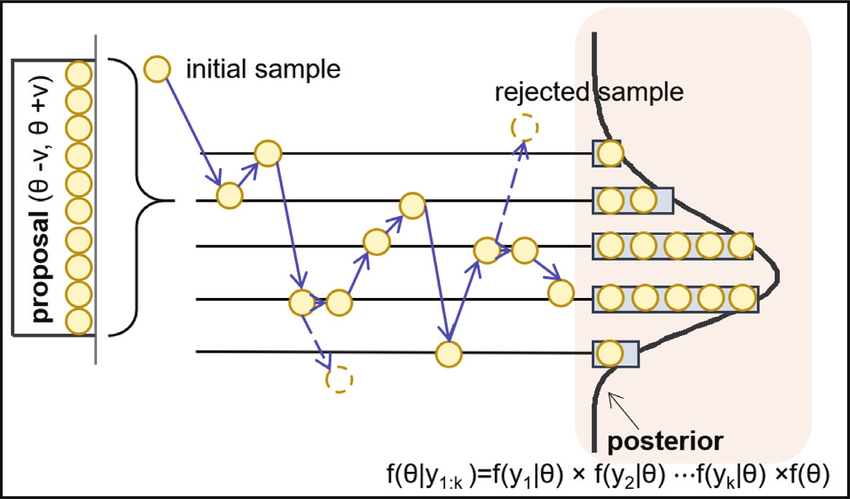
\includegraphics[width=0.75\linewidth]{Figures/mcmc1.png}

  \footnotesize{Dong T, An D, Kim NH. Prognostics 102: efficient Bayesian-based prognostics algorithm in Matlab. Fault Detection, Diagnosis and Prognosis. 2019 Feb 20:5-25.}
\end{frame}



\begin{frame}{MC vs. Metropolis--Hastings (layman comparison)}
  \begin{columns}[T,onlytextwidth]
    \column{0.48\textwidth}
    \textbf{MC (plain Monte Carlo)}
    \begin{itemize}
      \item You can already generate random samples from the distribution you care about.
      \item Each draw is independent of the last.
      \item Estimate an average by taking many draws and averaging.
    \end{itemize}

    \column{0.48\textwidth}
    \textbf{MH (Metropolis--Hastings)}
    \begin{itemize}
      \item You \emph{cannot} directly draw perfect samples from the posterior.
      \item You generate a sequence of guesses, where each new guess depends on the previous one.
      \item You keep moves that look better, and sometimes keep worse moves to avoid getting stuck.
    \end{itemize}
  \end{columns}

  \vspace{0.6em}
  \textbf{One-line takeaway:} MC is ``sampling is easy''; MH is ``sampling is hard, so we walk our way there''.
\end{frame}

\begin{frame}{MCMC: Metropolis--Hastings}
  \textbf{Goal:} sample from $p(\theta\mid \bm{x})$ when we cannot sample i.i.d. directly.

  \vspace{0.4em}
  \textbf{Algorithm (random-walk MH):}
  \begin{enumerate}
    \item Start at $\theta^{(0)}$.
    \item Propose $\theta'\sim r(\theta'\mid \theta^{(t)})$ (e.g., $\mathcal{N}(\theta^{(t)},\sigma^2 I)$).
    \item Accept with probability
      \[
        \alpha=\min\!\left(1,\frac{p(\bm{x}\mid \theta')\,p(\theta')\,r(\theta^{(t)}\mid \theta')}
        {p(\bm{x}\mid \theta^{(t)})\,p(\theta^{(t)})\,r(\theta'\mid \theta^{(t)})}\right).
      \]
    \item Set $\theta^{(t+1)}=\theta'$ if accepted, else $\theta^{(t+1)}=\theta^{(t)}$.
  \end{enumerate}

  \vspace{0.4em}
  \textbf{Key point:} the chain has stationary distribution $p(\theta\mid \bm{x})$ (after burn-in).
\end{frame}

\begin{frame}{MCMC: illustration}
  \centering
  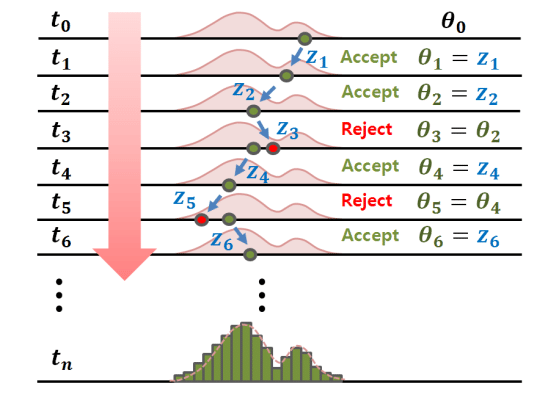
\includegraphics[width=0.7\linewidth]{Figures/mcmc.png}
\end{frame}



\begin{frame}{MCMC knobs (what to tune in practice)}
  \textbf{MCMC has ``knobs'' that trade off speed vs.\ accuracy.} Common ones:
  \begin{itemize}
    \item \textbf{Warm-up / burn-in:} initial iterations to let the chain reach the typical set;
          discard these samples.
    \item \textbf{Proposal / step size (MH):} too small $\Rightarrow$ slow exploration;
          too large $\Rightarrow$ low acceptance.
    \item \textbf{Number of iterations:} more draws reduce Monte Carlo error (but not bias from non-convergence).
    \item \textbf{Number of chains:} run multiple independent chains to assess convergence ($\hat{R}$) and robustness.
    \item \textbf{Thinning (optional):} keep every $k$-th draw; rarely needed.
  \end{itemize}


\end{frame}


\begin{frame}{Gibbs sampling (special case of MCMC)}
  \textbf{When it works well:} you can sample each conditional distribution.

  \vspace{0.4em}
  For $\theta=(\theta_1,\ldots,\theta_d)$, iterate:
  \[
    \theta_1^{(t+1)}\sim p(\theta_1\mid \theta_2^{(t)},\ldots,\theta_d^{(t)},\bm{x}),\;\;
    \ldots,\;\;
    \theta_d^{(t+1)}\sim p(\theta_d\mid \theta_1^{(t+1)},\ldots,\theta_{d-1}^{(t+1)},\bm{x}).
  \]

  \vspace{0.4em}
  \begin{itemize}
    \item Produces \textbf{correlated} samples, but targets the true posterior.
    \item Common in hierarchical Bayesian models (e.g., patient-level random effects).
  \end{itemize}
\end{frame}

\begin{frame}{Gibbs sampling: algorithm}
  \textbf{Goal:} draw samples from $p(\theta\mid \bm{x})$ by iteratively sampling full conditionals.

  \vspace{0.4em}
  \textbf{Setup:} choose an initial state $\theta^{(0)}=(\theta^{(0)}_1,\ldots,\theta^{(0)}_d)$.

  \vspace{0.2em}
  \textbf{For $t=0,1,\ldots,T-1$:}
  \begin{enumerate}
    \item For $j=1,\ldots,d$, sample
      \[
        \theta^{(t+1)}_j \sim p\!\left(\theta_j \mid \theta^{(t+1)}_{1:j-1},\,\theta^{(t)}_{j+1:d},\,\bm{x}\right).
      \]
    \item (Optional) record $\theta^{(t+1)}$ after warm-up / thinning.
  \end{enumerate}


\end{frame}

\begin{frame}{MC vs MCMC vs Gibbs}
  \centering
  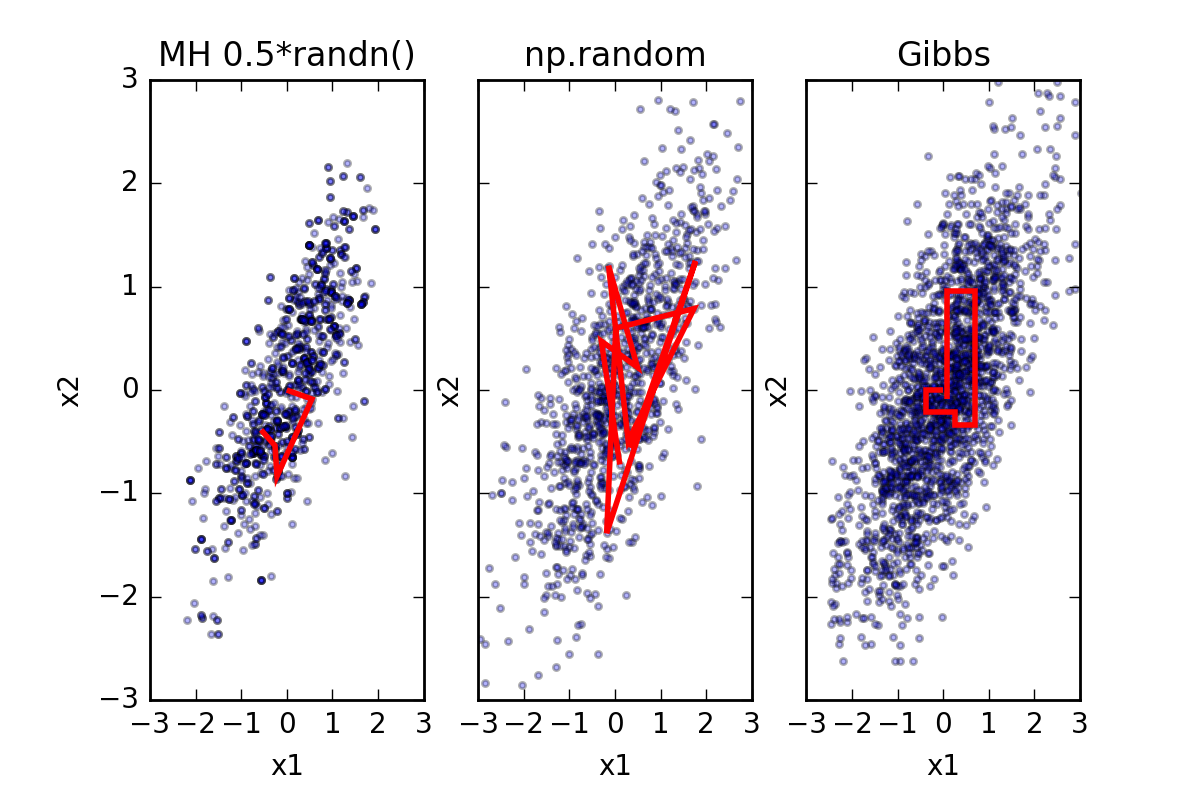
\includegraphics[width=0.7\linewidth]{Figures/BN_MH_vs_Gibbs.png}
  \footnotesize{http://algorithm-interest-group.com/algorithm/Gibbs-Sampling-Yubo-Paul-Yang/}
\end{frame}




%%%%%%%%%%%%%%%%%%%%%%%%%%%%%%%%%%%%%%%%%%%%%%%%%%%%%%%%%%%%%%%%%%%%%%%%%%
%%%%%%%%%%%%%%%%%%%%%%%%%%%%%%%%%%%%%%%%%%%%%%%%%%%%%%%%%%%%%%%%%%%%%%%%%%
%%%%%%%%%%%%%%%%%%%%%%%%%%%%%%%%%%%%%%%%%%%%%%%%%%%%%%%%%%%%%%%%%%%%%%%%%%

\begin{frame}[plain]
    \centering
    \vfill
    {\usebeamerfont{section title}Variational inference (VI) \par}
    \vfill
  \end{frame}



\begin{frame}{Variational inference (VI): layman explanation}
  \textbf{Big idea:} instead of \emph{sampling} from the true posterior (often slow),
  we pick a simple, adjustable distribution and \emph{tune it} to look as much like the posterior as possible.

  \vspace{0.4em}
  \begin{itemize}
    \item Think of the true posterior as a complicated shape we cannot work with directly.
    \item We choose a simpler shape (often a Gaussian, or a factorized family) with knobs $\phi$.
    \item We turn the knobs so the simple shape covers the high-probability region well.
    \item Result: fast approximate uncertainty (but it can miss tails / correlations).
  \end{itemize}
  https://www.youtube.com/watch?v=A9WmgK9qpm0
\end{frame}

\begin{frame}{VI}
  \centering
  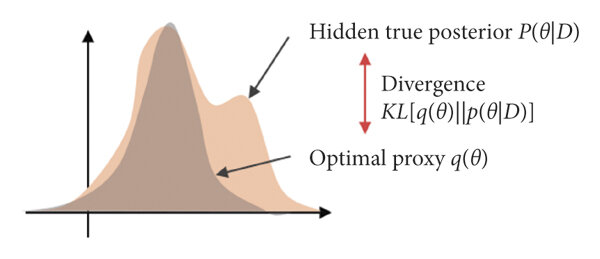
\includegraphics[width=0.9\linewidth]{Figures/vi2.png}
  \footnotesize{https://doi.org/10.1155/2020/7897824}
\end{frame}


\begin{frame}{VI intuition: like fitting a flexible blanket}
  \textbf{Analogy:} the posterior is an uneven landscape; VI is like placing a flexible blanket on top.
  \begin{itemize}
    \item The blanket shape is $q_\phi(\theta)$ (simple family).
    \item You adjust it to sit tightly over the important valleys (high probability).
    \item The tighter it fits (higher objective), the closer $q_\phi$ is to the posterior.
  \end{itemize}

  \vspace{0.4em}
  \textbf{Takeaway:} VI turns inference into an \emph{optimization problem} (find best $\phi$),
  so it can use the same toolset as ML training (SGD, Adam, mini-batches).
\end{frame}




\begin{frame}{VI}
  \centering
  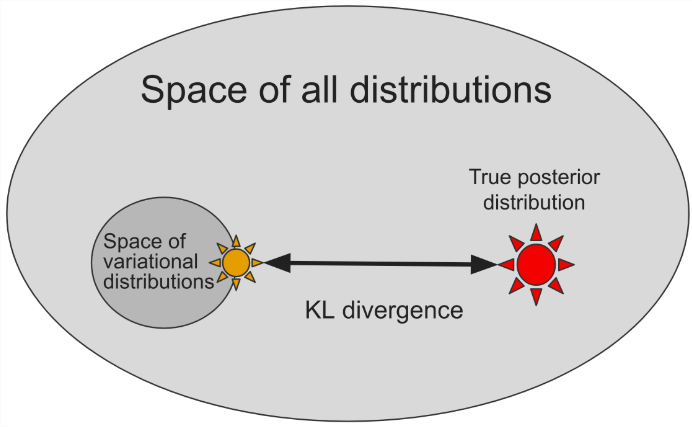
\includegraphics[width=0.7\linewidth]{Figures/vi1.png}

\end{frame}


\begin{frame}{Variational inference (VI)}
  \textbf{Idea:} approximate posterior $p(\theta\mid \bm{x})$ with a simpler family $q_\phi(\theta)$
  by solving an optimization problem.
  \[
    q_{\phi}^\star
    =
    \arg\min_{q_\phi \in \mathcal{Q}}
    \mathrm{D_{KL}}\!\left(q_\phi(\theta)\,\|\,p(\theta\mid \bm{x})\right)
    \;\;\Longleftrightarrow\;\;
    \arg\max_{\phi}\ \mathrm{ELBO}(\phi).
  \]
  \begin{itemize}
    \item \textbf{Pros:} fast, scalable (mini-batches), good for large datasets.
    \item \textbf{Cons:} biased approximation; common KL direction can \emph{underestimate} uncertainty.
    \item \textbf{Variants:} mean-field VI, structured VI, amortized VI (VAEs), black-box VI.
  \end{itemize}
\end{frame}

\begin{frame}{VI}
  \centering
  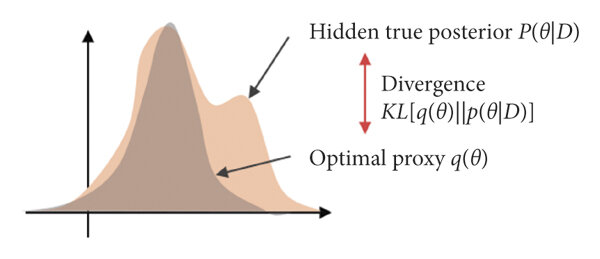
\includegraphics[width=0.9\linewidth]{Figures/vi2.png}
  \footnotesize{https://doi.org/10.1155/2020/7897824}
\end{frame}

% ----------------------------- ELBO slides ----------------------------- %
\begin{frame}{ELBO: objective and why we need it}
  \textbf{Goal:} approximate the intractable posterior $p(\theta\mid \bm{x})$ with $q_\phi(\theta)$.

  \vspace{0.4em}
  \textbf{Natural objective:} minimize the KL divergence
  \[
    D_{\mathrm{KL}}\!\left(q_\phi(\theta)\,\|\,p(\theta\mid \bm{x})\right)
    =
    \mathbb{E}_{q_\phi}\!\left[\log\frac{q_\phi(\theta)}{p(\theta\mid \bm{x})}\right].
  \]

  \vspace{0.2em}
  \textbf{Problem:} $p(\theta\mid \bm{x})=\dfrac{p(\bm{x},\theta)}{p(\bm{x})}$ depends on
  $p(\bm{x})=\int p(\bm{x},\theta)\,d\theta$, which is typically intractable.
\end{frame}

\begin{frame}{From KL to ELBO (derivation)}
  Start with
  \[
    D_{\mathrm{KL}}\!\left(q_\phi(\theta)\,\|\,p(\theta\mid \bm{x})\right)
    =
    \mathbb{E}_{q_\phi}[\log q_\phi(\theta)]-\mathbb{E}_{q_\phi}[\log p(\theta\mid \bm{x})].
  \]
  Substitute $\log p(\theta\mid \bm{x})=\log p(\bm{x},\theta)-\log p(\bm{x})$:
  \[
    D_{\mathrm{KL}}(q\,\|\,p(\cdot\mid \bm{x}))
    =
    \mathbb{E}_{q_\phi}[\log q_\phi(\theta)]-\mathbb{E}_{q_\phi}[\log p(\bm{x},\theta)]+\log p(\bm{x}).
  \]

  Rearranging gives the ELBO:
  \[
    \log p(\bm{x})
    =
    \underbrace{\mathbb{E}_{q_\phi}[\log p(\bm{x},\theta)]-\mathbb{E}_{q_\phi}[\log q_\phi(\theta)]}_{\mathrm{ELBO}(\phi)}
    +
    D_{\mathrm{KL}}\!\left(q_\phi(\theta)\,\|\,p(\theta\mid \bm{x})\right).
  \]
\end{frame}



\begin{frame}{ELBO: equivalent forms (interpretation)}

  $$\mathrm{ELBO}(\phi) = \mathbb{E}_{q_\phi}[\log p(\bm{x},\theta)]-\mathbb{E}_{q_\phi}[\log q_\phi(\theta)]$$

  Using $p(\bm{x},\theta)=p(\bm{x}\mid \theta)p(\theta)$:
  \[
    \mathrm{ELBO}(\phi)
    =
    \mathbb{E}_{q_\phi}[\log p(\bm{x}\mid \theta)]
    +\mathbb{E}_{q_\phi}[\log p(\theta)]
    -\mathbb{E}_{q_\phi}[\log q_\phi(\theta)].
  \]
  Equivalently,
  \[
    \mathrm{ELBO}(\phi)
    =
    \mathbb{E}_{q_\phi}[\log p(\bm{x}\mid \theta)]
    -
    D_{\mathrm{KL}}\!\left(q_\phi(\theta)\,\|\,p(\theta)\right).
  \]

  \vspace{0.2em}
  \textbf{Trade-off:}
  \begin{itemize}
    \item \textbf{Data fit term} $\mathbb{E}_{q_\phi}[\log p(\bm{x}\mid \theta)]$ (reconstruction / expected log-likelihood)
    \item \textbf{Regularizer} $-D_{\mathrm{KL}}(q_\phi(\theta)\,\|\,p(\theta))$ (keep $q_\phi$ close to the prior)
  \end{itemize}
\end{frame}



\begin{frame}{Choosing the Variational Family $q_\phi(\theta)$}
  The choice of $q$ impacts the accuracy vs.\ efficiency trade-off.

  \vspace{0.3em}
  \textbf{1. Fixed-Form VI:}
  Assume $q_\phi(\theta)$ belongs to a parametric family (e.g., Gaussian).


  \vspace{0.3em}
  \textbf{2. Free-Form VI (Mean-Field Approximation):}
  Assume $q$ factorizes over groups of variables:
  $$ q(\theta) = \prod_{j=1}^{J} q_j(\theta_j) $$

\end{frame}

\begin{frame}{1. Fixed-Form Variational Inference}
    \begin{columns}
        \begin{column}{0.55\textwidth}
            \textbf{Assumption:} $q_\phi(\theta)$ belongs to a parametric family.
            
            \vspace{0.5em}
            \textbf{Gaussian Family:}
            $$ q_\phi(\theta) = \mathcal{N}(\theta \mid \bm{\mu}, \bm{\Sigma}) $$
            \begin{itemize}
                \item \emph{Pros:} Simple optimization; matches if posterior is truly Gaussian.
                \item \emph{Cons:} 
                \begin{itemize}
                    \item Cannot capture multi-modality or skew.
                    \item Full $\bm{\Sigma}$ is $O(D^2)$ (computationally expensive).
                \end{itemize}
            \end{itemize}
        \end{column}
        
        \begin{column}{0.45\textwidth}
            \centering
            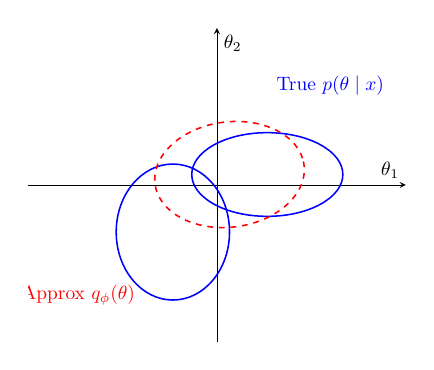
\begin{tikzpicture}[scale=0.7]
              \begin{axis}[
                ticks=none,
                axis lines=middle,
                xlabel=$\theta_1$, ylabel=$\theta_2$,
                xmin=-3, xmax=3, ymin=-3, ymax=3,
                view={0}{90},
                enlargelimits=false
              ]
                % NOTE: pgfplots' `contour gnuplot` requires shell-escape (disabled on many online compilers),
                % which results in an empty plot. Use explicit contour ellipses instead (fully TeX-native).
                \draw[blue, thick]
                  (axis cs:0.8,0.2) ellipse [x radius=1.2, y radius=0.8];
                \draw[blue, thick]
                  (axis cs:-0.7,-0.9) ellipse [x radius=0.9, y radius=1.3];

                % Gaussian approximation: plot a rotated ellipse inside the axis coordinates.
                \addplot[
                  red, thick, dashed,
                  domain=0:360, samples=181
                ]
                ({0.2 + 1.2*cos(x)*cos(15) - 1.0*sin(x)*sin(15)},
                 {0.2 + 1.2*cos(x)*sin(15) + 1.0*sin(x)*cos(15)});

                % Labels
                \node[blue] at (axis cs: 1.8, 1.9) {True $p(\theta\mid x)$};
                \node[red]  at (axis cs: -2.2, -2.1) {Approx $q_\phi(\theta)$};
              \end{axis}
            \end{tikzpicture}
            \vspace{0.2em}
            \footnotesize{\textcolor{blue}{Complex Posterior} vs \textcolor{red}{Gaussian Approx}}
        \end{column}
    \end{columns}
\end{frame}

\begin{frame}{2. Free-Form VI (Mean-Field Approximation)}
    \begin{columns}
        \begin{column}{0.55\textwidth}
            \textbf{Assumption:} $q$ factorizes over variables.
            $$ q(\theta) = \prod_{j=1}^{J} q_j(\theta_j) $$
            
            \vspace{0.5em}
            \textbf{Key Characteristics:}
            \begin{itemize}
                \item \textbf{Pros:} Flexible; no specific form assumed for factors $q_j$.
                \item \textbf{Cons:} \textbf{Ignores correlations}.
                \item \emph{Result:} Often underestimates variance (see diagram).
            \end{itemize}
        \end{column}
        
        \begin{column}{0.45\textwidth}
            \centering
            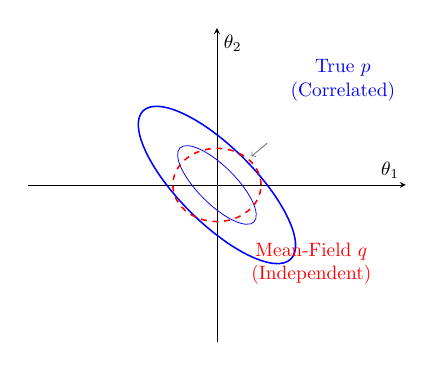
\begin{tikzpicture}[scale=0.7]
                \begin{axis}[
                    ticks=none,
                    axis lines=middle,
                    xlabel=$\theta_1$, ylabel=$\theta_2$,
                    xmin=-3, xmax=3, ymin=-3, ymax=3
                ]
                
                % 1. True Posterior with Correlation (Rotated Ellipse)
                \draw[blue, thick] (axis cs:0,0) ellipse [x radius=0.6, y radius=2, rotate=45];
                \draw[blue, thin] (axis cs:0,0) ellipse [x radius=0.3, y radius=1, rotate=45];
                
                % 2. Mean Field Approximation (Axis Aligned)
                % It must be axis aligned because q(t1)q(t2) implies independence
                \draw[red, thick, dashed] (axis cs:0,0) circle [radius=0.7];
                
                % Labels
                \node[blue, align=center] at (axis cs: 2, 2) {True $p$\\ (Correlated)};
                \node[red, align=center] at (axis cs: 1.5, -1.5) {Mean-Field $q$\\ (Independent)};
                
                % Arrow highlighting the gap
                \draw[->, black!60, shorten >=2pt] (axis cs:0.8, 0.8) -- (axis cs: 0.5, 0.5);
                
                \end{axis}
            \end{tikzpicture}
            \vspace{0.2em}
            \footnotesize{Mean-field forces \textbf{axis-alignment}}
        \end{column}
    \end{columns}
\end{frame}

\begin{frame}{Optimization Techniques in VI}
  We typically maximize the ELBO using one of two classes of methods:

  \vspace{0.4em}
  \textbf{1. Coordinate Ascent (CAVI)}
  \begin{itemize}
    \item Update each factor $q_j(\theta_j)$ (or parameter subset) while holding others fixed.
    \item Derives closed-form updates; commonly used with the \textbf{Mean-Field} approximation.
  \end{itemize}

  \vspace{0.4em}
  \textbf{2. Gradient-Based Methods}
  \begin{itemize}
    \item Utilize gradients $\nabla_{\phi} \mathrm{ELBO}$ to iteratively update parameters.
    \item \textbf{Stochastic Gradient Descent (SGD):} Updates based on mini-batches of data.
    \item Methods like Adam or RMSprop are standard for \textbf{Black-Box VI} and \textbf{VAEs}.
  \end{itemize}
\end{frame}

\begin{frame}[plain]
    \centering
    \vfill
    {\usebeamerfont{section title}Application: Bayesian Neural Networks (BNNs) \par}
    \vfill
\end{frame}






\end{document}